\documentclass{article}
\usepackage{longtable}
\usepackage{graphicx}
\usepackage{float} 
\usepackage{amsmath}



\begin{document}
\section*{Supplemental Information}
REWRITE FOR 13-18
\section{Introduction: Rare events and unofficial data}

The analyses in this paper seek to simultaneously address two significant methodological challenges. The first is the relatively rarity of police-involved killings for many age-sex-race specific subgroups with small national populations. The second is the absence of valid official data. Below, we discuss our approach to maximizing the available information for life table estimates in addition to evaluating the validity of Fatal Encounters, the unofficial source of data on police-involved deaths used in this analysis. 

First, Police killings are a relatively rare event for many race-age-sex specific subgroups. For example, Asian/Pacific Islander women were killed by police at a rate of about $1.7 \times 10^{-7}$ per 100,000 persons between 2008 and 2018. In 2017, the American Community Survey reports a population of Asian/Pacific-Islander women between the ages of 50 and 54 of $666102$. At that rate, we expect to observe an average of about 0.1 deaths per year in this age group. Relying on any single year for life table estimates would produce a misleading estimate for age-specific risk estimate for this group; either zero or an order of magnitude higher than our calculated estimate. By pooling all years of valid data, we are able to include dramatically more information in our life table estimates. However, by doing so, we are forced to make potentially problematic assumptions about the stability of age-specific risk over time and the stability of differences in risk across groups over time. Below, we describe the nature of temporal trends in the data, and motivate our approach to accounting for these trends while still maximizing information on this rare event. We pursue a model-based approach that relies on posterior prediction for life table estimation of risk. This approach simultaneously smooths temporal trends and incorporates uncertainty driven by temporal variation into our findings. 

Second, there are currently no nationally comprehensive official sources of data on police-involved killings. The Bureau of Justice Statistics acknowledged the limitations of their Arrest-Related Deaths data collection effort, and ceased data collection in 2014 (CITATIONS). The National Vital Statistics System (NVSS), the nation's key source of mortality data is known to undercount law enforcement related deaths (CITATIONS). The National Violent Death Reporting System (NVDRS) has far better coverage of police-involved deaths than does NVSS (CITATIONS), but currently lacks the geographic and temporal coverage needed to generate national estimates. Despite widespread calls for better data on police-involved deaths (CITATIONS), government agencies have systematically failed to design and implement an adequate system to track police-involved deaths, or more generally, officer use-of-force. Journalists and independent researchers have stepped into this gap. Following the rise of the Black Lives Matter movement and increasing attention paid to police killings of people of color in the mid 2010s, multiple projects emerged to use public records and media reports to systematically document police violence. Among these novel data collection efforts, Fatal Encounters has the broadest temporal scope and broadest inclusion criteria for police-involved deaths. Where other efforts have focused exclusively on shootings or a narrow subset of years, Fatal Encounters seeks to include all cases in which police were in any way involved in a death of a civilian between January 1, 2000 and the present, with the important exception of deaths occurring in custody (that is after an arrestee has been formally booked into a jail or other detention facility). These unofficial data have been widely used in descriptive and inferential social science research (CITATIONS) and have been found to have good coverage of cases recorded in official data systems (CITATIONS). 

Below, we describe our methods for evaluating the validity of Fatal Encounters data and our approach to addressing the challenges of estimating risk for rare events in contexts when underlying risk is likely changing over time. THIS APPENDIX PROCEEDS IN N SECTIONS. BRIEF SUMMARY OF EACH.

\section{Validity of Fatal Encounters between 2000 and 2018}

FATAL ENCOUNTERS - WHY DID WE CHOOSE AND WHAT IS ITS METHOD

WHY STOP IN 18? Mostly for pop data reasons

\subsection{Internet news and undercounts of cases}

Fatal Encounters data is available for cases between 2000 and 2019, with new cases being added to the dataset on an ongoing basis. Here, we consider whether Fatal Encounters provides reliable data on counts of deaths involving police across the full period included in the dataset. 

We suspect that the data undercount police-involved deaths in periods prior to 2007. The primary collector of the Fatal Encounters data, D. Brian Burghart, believes that the lack of local online news publication as well as the routine practice of purging archived internet content prior to the advent of inexpensive cloud storage has led to a significant undercount of cases between 2000 and 2007.

Given Burghart's suspicion that the source data (searchable internet news coverage) is censored prior to 2007 as a function of the spread and accessibility of web news production and inexpensive storage, we suspect that data on general internet usage among the US population should correlate with an unobserved undercount of events recorded in Fatal Encounters. We obtain time series data on the rates of internet usage among US adults from the St. Louis Federal Reserve (World Bank, Internet users for the United States [ITNETUSERP2USA], retrieved from FRED, Federal Reserve Bank of St. Louis; https://fred.stlouisfed.org/series/ITNETUSERP2USA, February 15, 2019.), and compare this data to counts of police-involved deaths derived from Fatal Encounters by year in Figure \ref{fig:internet}.

\begin{figure}
	\centering
	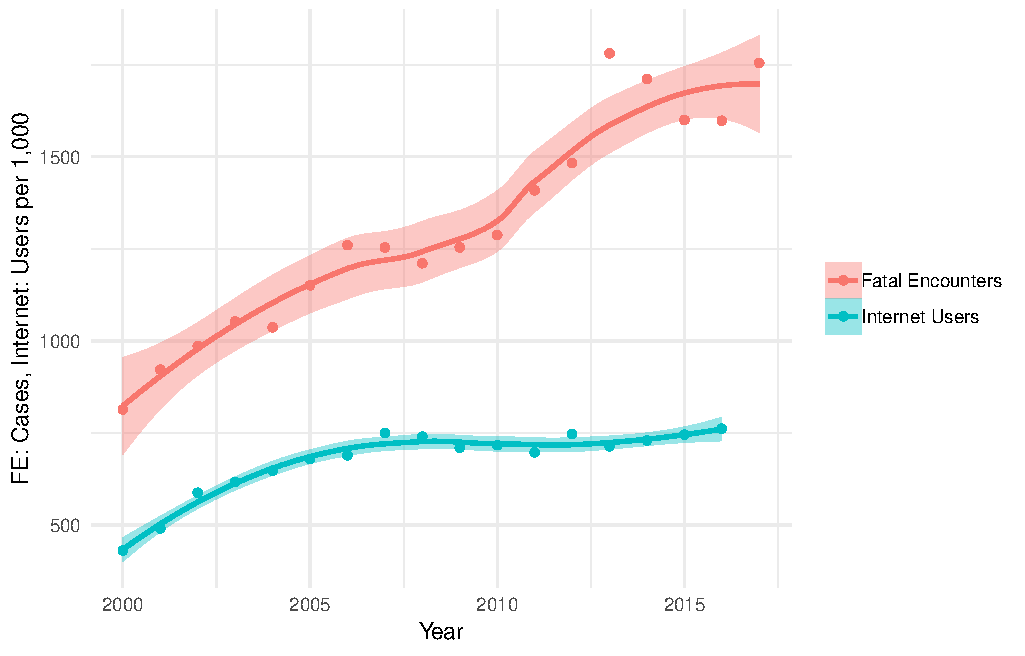
\includegraphics[width=\linewidth]{vis/internet_use_ts.pdf}
	\caption{Deaths recorded in Fatal Encounters and Internet users per 1,000 persons, 2000 to 2016.}
	\label{fig:internet}
\end{figure}

Figure \ref{fig:internet} shows a close correlation between the increasing use of the internet among Americans and the counts of deaths recorded in Fatal Encounters for the years 2000 through 2007. The trends appear to decouple after 2007. This is consistent with a censorship hypothesis. In earlier years of the data, there is likely a larger unobserved set of cases that are not accessible to Fatal Encounters researchers using their web-based search methodology than there is in later years of the data.

\subsection{Comparing trends in NVSS and Fatal Encounters}

The National Vital Statistics System provides a potential source for evaluating the external validity of Fatal Encounters data. The NVSS records the cause of death for all DEFINE NVSS SCOPE. ``Legal intervention'' is included among the codes for causes of death in NVSS. DEFINE THE CODE. Prior research has established that NVSS systematically undercounts officer-involved deaths (CITES). 

However, if we assume that there has been no change in the probability that officer-involved deaths are coded as ``legal intervention'' in NVSS over time, the observable time series trends in NVSS should be correlated with the true unobserved time series of police-involved deaths. With this assumption, we evaluate the time series of NVSS police-involved deaths and Fatal Encounters officer use-of-force deaths to further explore the possibility of censorship and gain insight into temporal trends in the risk of police-involved death. We display this time series in Figure \ref{fig:countTS}. Because NVSS under-reports officer-involved deaths, we provide a time series transformed to a proportional change in counts of deaths relative to the count of deaths in 2000 in each dataset in Figure \ref{fig:pctTS} to enable direct comparison of the two trends on a common scale. 

\begin{figure}
	\centering
	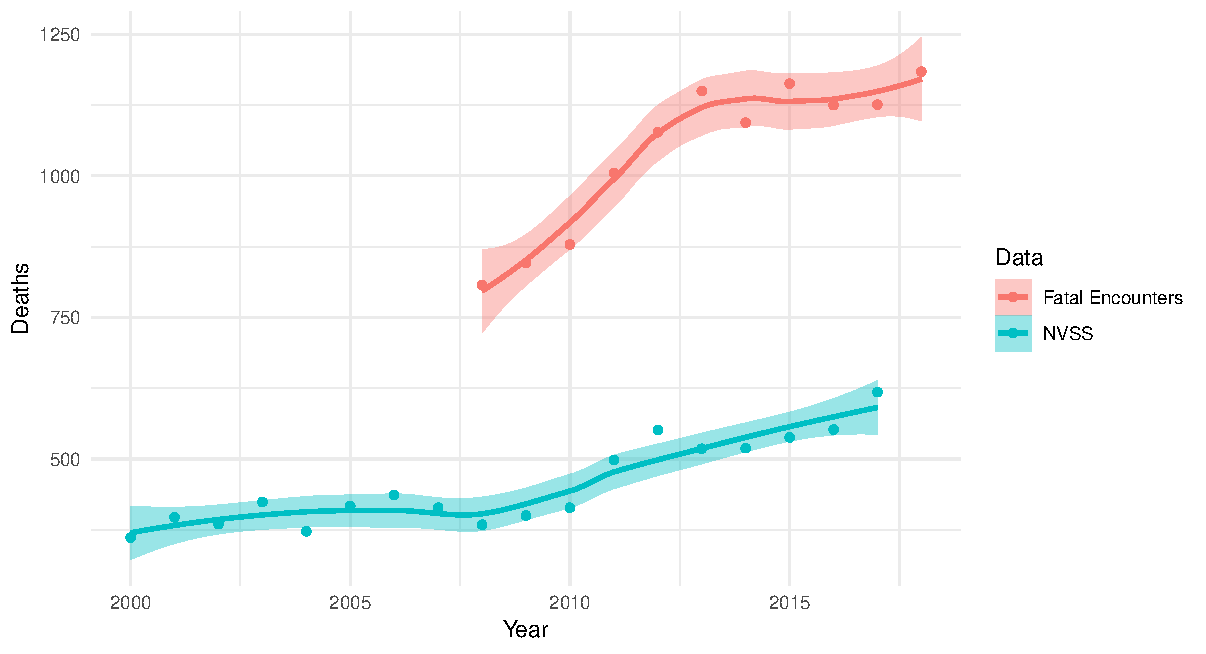
\includegraphics[width = \linewidth]{vis/nvss_fe_ts.pdf}
	\caption{Deaths due to officer use of force recorded in Fatal Encounters and NVSS 2000 to 2018}
	\label{fig:countTS}
\end{figure}

\begin{figure}
	\centering
	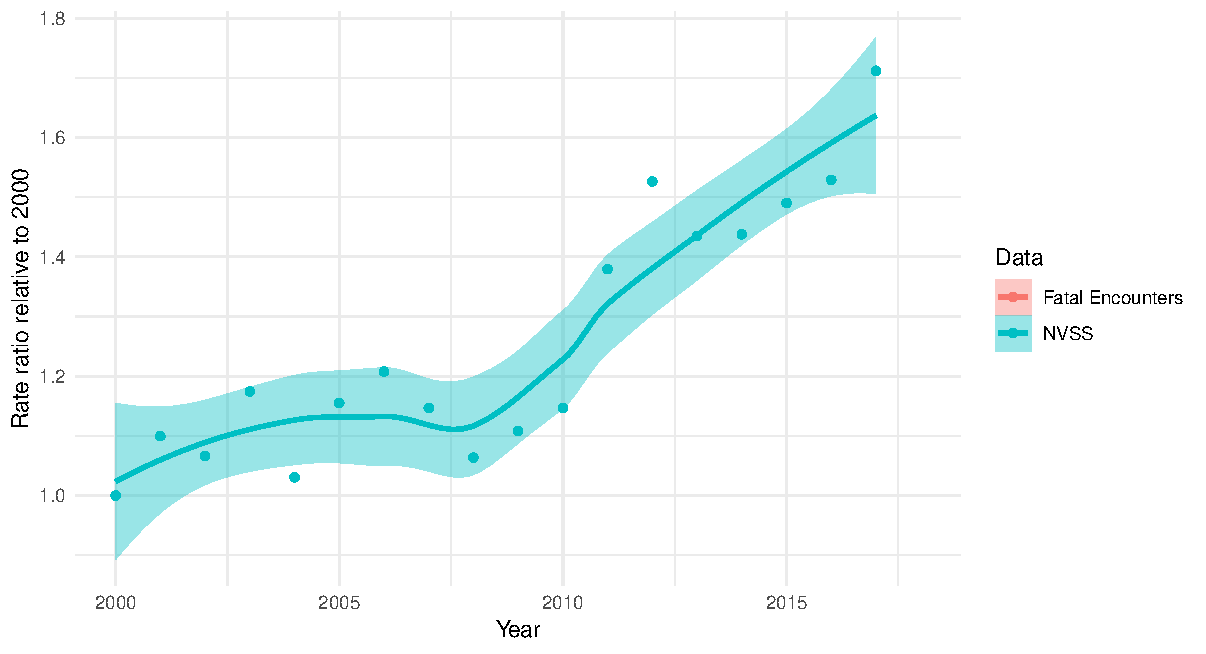
\includegraphics[width = \linewidth]{vis/nvss_fe_pct.pdf}
	\caption{Proportional change in reported deaths in NVSS and Fatal Encounters since 2000}
	\label{fig:pctTS}
\end{figure}

Figures \ref{fig:countTS} and \ref{fig:pctTS} show that counts of deaths reported in NVSS remained relatively stable between 2000 and 2010. During this time, rates fluctuated between 1.0 and 1.2 times the count of officer-involved deaths reported in 2000. Between 2011 and 2017 (the most recent available data), the count of cases in the data increased substantially. In 2017, there were about 1.7 times more legal intervention deaths reported in NVSS than there were in 2000. 

Fatal Encounters exhibits a relatively stable positive trend between 2000 and 2018. The magnitude of growth in cases recorded in FE over time is higher than for NVSS; for 2018, FE records about 2.3 times more deaths than it records for 2000. While this evidence is far from definitive, trends in the proliferation of internet access and the NVSS time series suggest that undercounts in Fatal Encounters due to unavailable online news records of officer-involved deaths likely decreased over time until approximately 2007. The shape of trends in Fatal Encounters and NVSS become more tightly linked between 2008 and 2017. 

\begin{figure}[H]
	\centering
	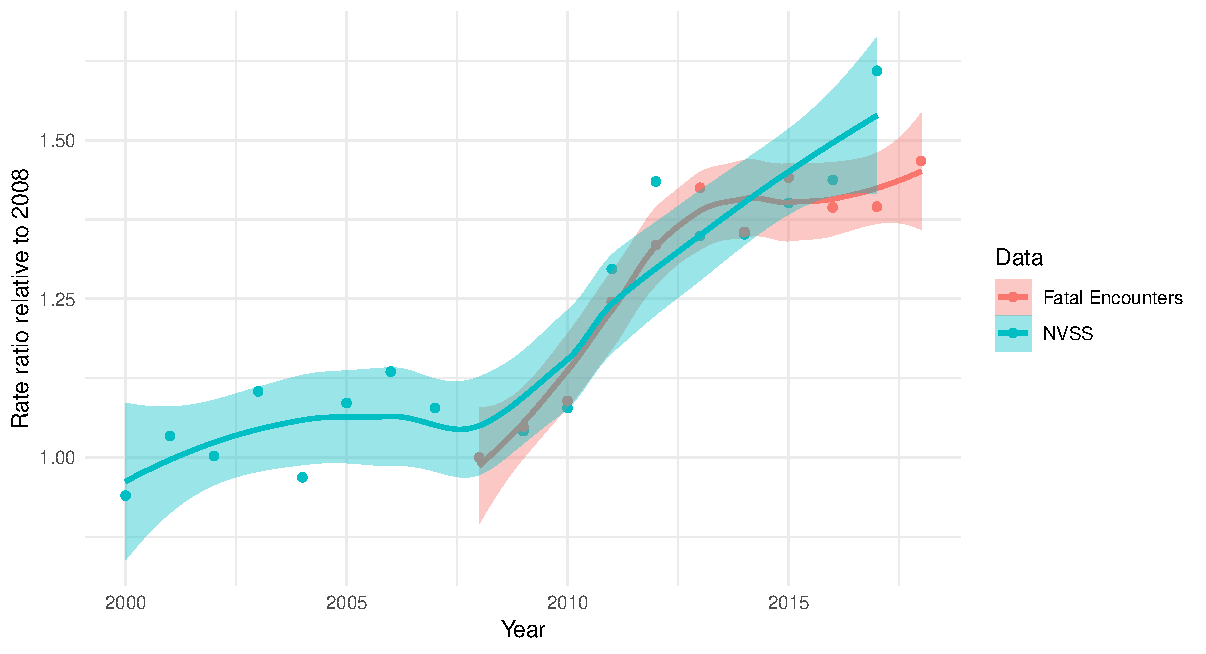
\includegraphics[width = \linewidth]{vis/nvss_fe_pct_08.pdf}
	\caption{Proportional change in reported deaths in NVSS and Fatal Encounters since 2008}
	\label{fig:pct_08}
\end{figure}

Figure \ref{fig:pct_08} rescales both time series to display proportional changes in case counts relative to the observed counts for 2008. This figure strongly suggests that the trends in NVSS and Fatal Encounters converge after 2008. It may be fruitful in future research to estimate the magnitude of undercoverage in FE using secondary data like NVSS. Based on this analysis, in this paper we assume that undercoverage in Fatal Encounters becomes less pronounced after 2007, and focus our analyses on cases recorded as occurring between 2008 and 2018. 

\section{Models of temporal variation in group-specific risk}

% As shown in figure \ref{fig:pct_08}, there has been an increase in police-involved killings between 2008 and 2018. 

% SAY MORE ON LIFE TABLE ASSUMPTIONS ON RISK - ASSUMPTION ISNT THAT RISK IS STABLE, BUT THAT AGE-RISK PATTERNS ARE STABLE, RIGHT? THINK HARD ON THIS

% This relatively steep increase in the prevalence of police-involved killings may bias our estimates of the lifetime risk of being killed by police

% INCLUDE MIKE'S PLOTS. SAY THAT WE'RE MODELING AND SIMULATING TO NET OUT TIME TRENDS FOR NEW TABLES. SHOULD BE MORE ROBUST TO WITHIN-PERIOD CHANGES

% THIS IS A PROBLEM - 

% 1. Do a 13-18 table
% 2. Do a 08-18 table
% 3. Show the model-predicted table

% Be exceptionally clear about AT CURRENT RATES throughout paper, tamp down lifetime risk. 

To systematically incorporate information from multiple years of \textit{Fatal Encounters} data into our life table estimates, we build Bayesian negative binomial regression models of police-involved deaths with year, race, sex, and age as predictors. We use these models to predict group-specific risks of being killed by police by for a year \textit{unobserved} in the data. (Our prediction for a new year represents our best estimate of police-homicide risk for each demographic group, synthesized from the available data.) 

We assume---and confirm, later, via model comparison tests---that police-homicide risk varies jointly by age, sex and race. To appropriately incorporate time---which has a more ambiguous functional relationship with police-homicide risk---into our predictions, we first examine how police-homicides vary across years in the observed data.  

In the observed data, a time-trend in total death count is apparent. Figure \ref{fig:a1} displays a plot of the count of police-involved deaths, for each sex and race group, as a function of time: 

\begin{figure}[H]
	\centering
	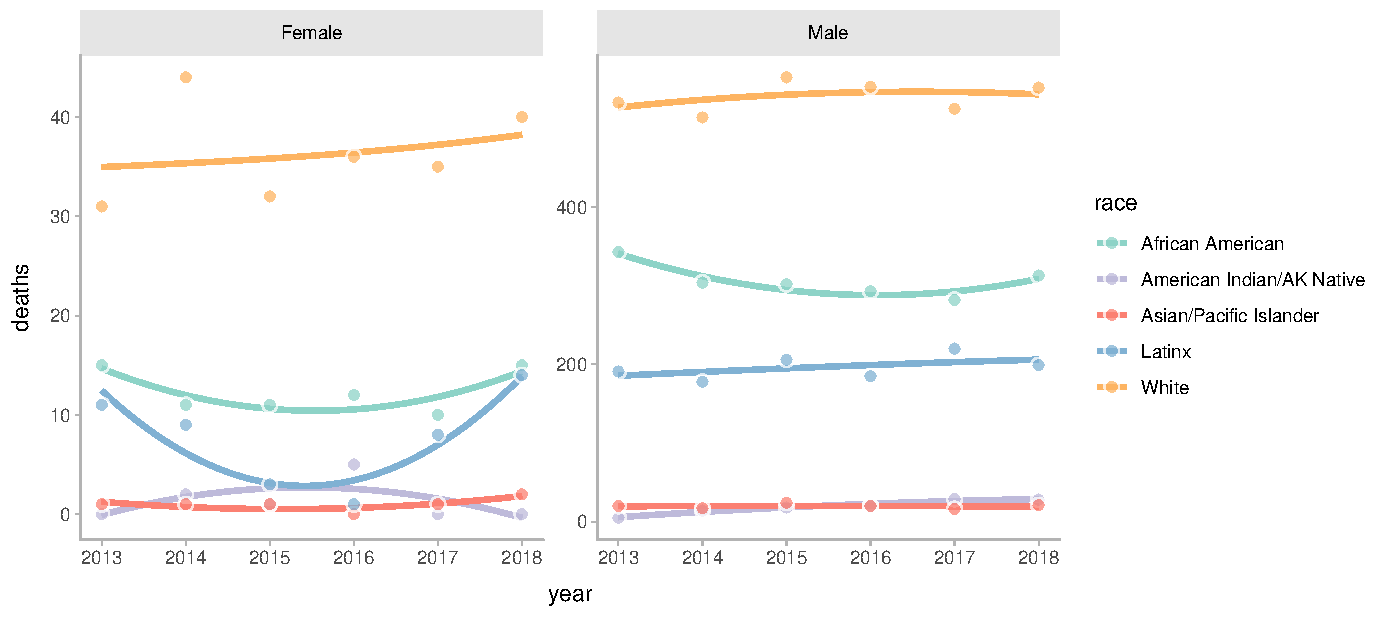
\includegraphics[width = \linewidth]{vis/fig_a1.pdf}
	\caption{Observed count of police-involved deaths, by race and sex, 2008-2018.}
	\label{fig:a1}
\end{figure}

For most groups in the data, the observed count of police involved deaths stays table from 2008-2018. Among Whites, however, total counts do increase over time. 

While time effects appear to vary by race, age (and sex) specific effects appear to be relatively consistent across time. Figures \ref{fig:a2} and \ref{fig:a3} display the observed relationship among age, race, sex, and count of police-homicides across each year of the data:

\begin{figure}
	\centering
	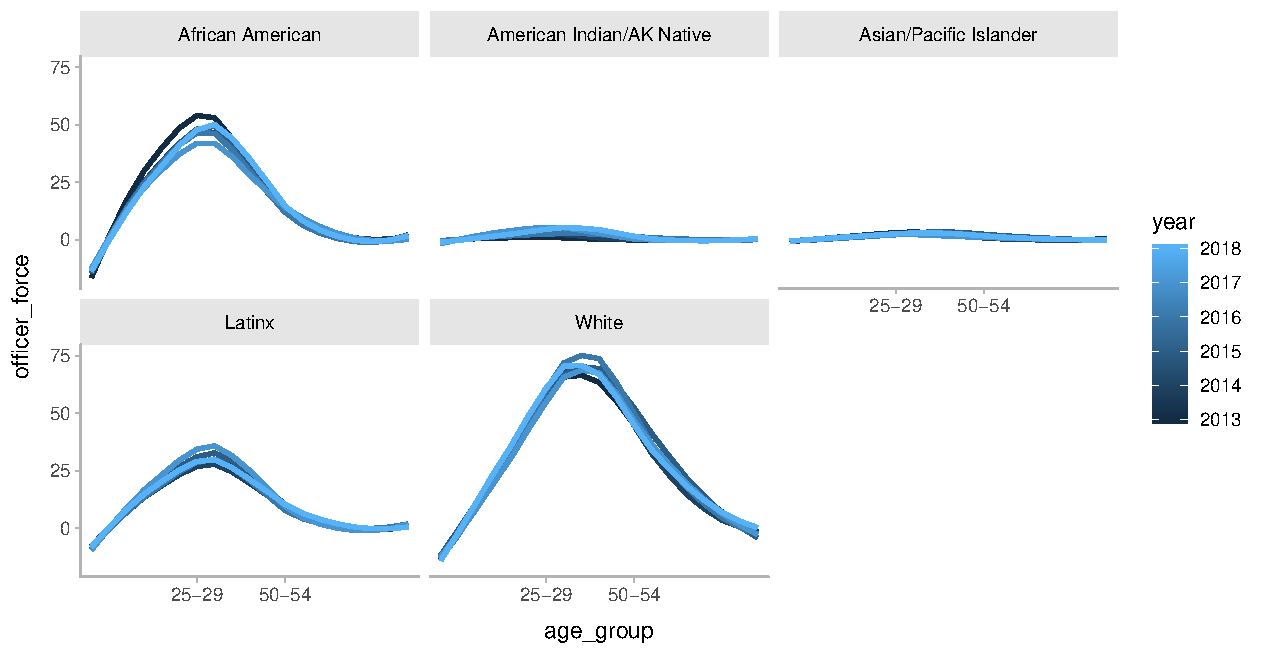
\includegraphics[width = \linewidth]{vis/fig_a2.pdf}
	\caption{Males: Observed count of police-involved deaths, by age, race, sex, and year. Note: curves are produced via a loess smooth of the observed data.}
	\label{fig:a2}
\end{figure}

\begin{figure}
	\centering
	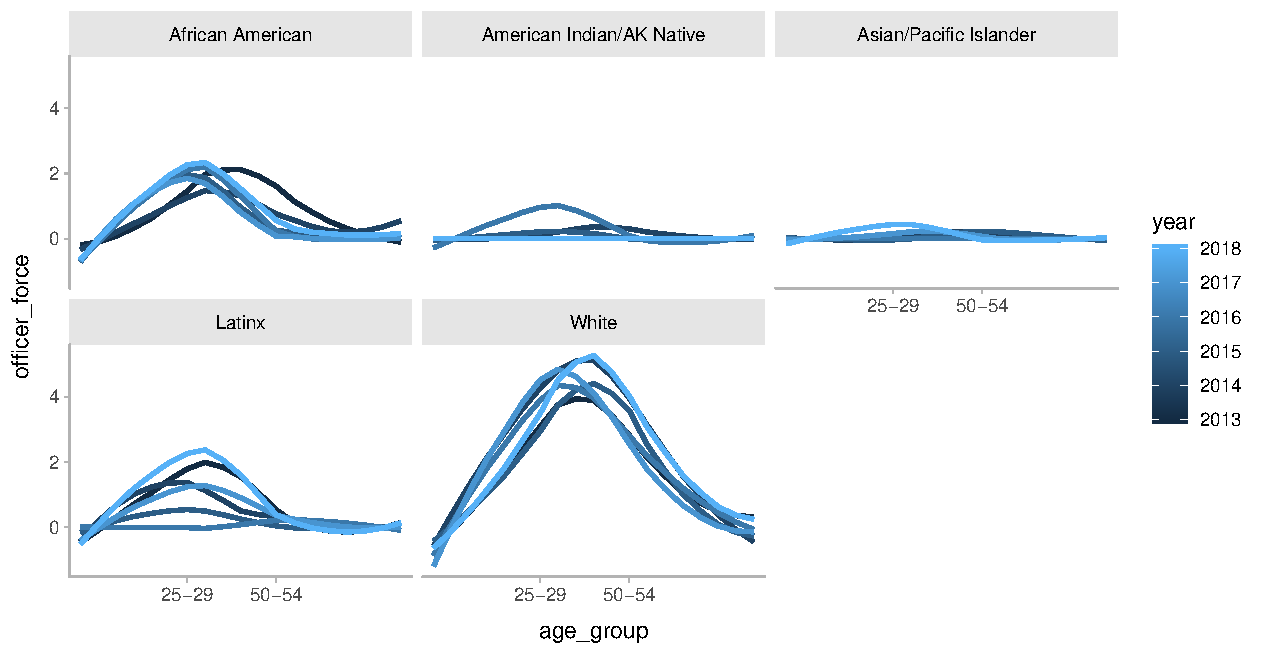
\includegraphics[width = \linewidth]{vis/fig_a3.pdf}
	\caption{Females: Observed count of police-involved deaths, by age, race, sex, and year. Note: curves are produced via a loess smooth of the observed data.}
	\label{fig:a3}
\end{figure}

Among males, the age-specific risk of being killed by police is stable across years among all groups. (E.g., among White males, a year-based intercept shift is apparent---in that, as shown above, more recent years display higher overall counts---but the age at which White men are most at risk of being killed by police remains constant across time.) Patterns among females are somewhat more variable across years; the very small counts among these groups, however, make it difficult to tell the degree to which this variation is due to noise.

Taken together, the observed data suggests that a model allowing year effects to vary among racial groups might provide a more accurate prediction of one's risk of being killed by police, in a new year, than a model that fixes the year-to-year variation in deaths counts to be equal among racial groups. 

The observed data also suggest that the risk of being killed by police across age groups is largely independent of year. (E.g., while the total count of deaths vary by race across years, the age pattern observed within each group remains stable across time.) To further interrogate this assumption about stability---particularly among females---we build a second set of regression models that allow for time effects to vary by race, age, and sex. To reduce the number of parameters needed to estimate this 4-way interaction, we treat both age and year effects as interval measures and stratify the sample by race and sex. For each race-by-sex subset of the data, we first regress death counts on age and year---with both predictor variables modeled as splines to capture the unknown, likely nonlinear, form of the relationship among these measures and mortality risk (i.e., Model A). Second, we estimate a bivariate spline for age and year, to allow for mortality risk to vary jointly by year and age for each race-by-sex group (i.e., Model B). We compare and combine models using Bayesian stacking weights (Yao et. al. 2018). This method allows us to use information provided by both models, weighted by their accuracy in leave-one-out cross-validation test. (Posterior predictions from models that provide more accurate predictions of the data are given more weight in this scheme.) 

Results for males confirm the patterns in the observed data: for all groups examined, the model that excluded a year-by-age interaction was assigned 100 percent of the stacking weight. (This suggest that the interaction among age and year provides little useful information for making predictions among males.) Among females, models without a year-by-age interaction were also more highly weighted---thus indicating better predictive performance---but not did not entirely dominate the model space. For instance, among Black females, the model without a year by age interaction received a 81 percent weight, while the model that included said interaction received 19 percent of the stacking weight. Figure \ref{fig:a4} plots the predictions generated from both models for Black females, as well as predictions generated from their combined posteriors. 


\begin{figure}
	\centering
	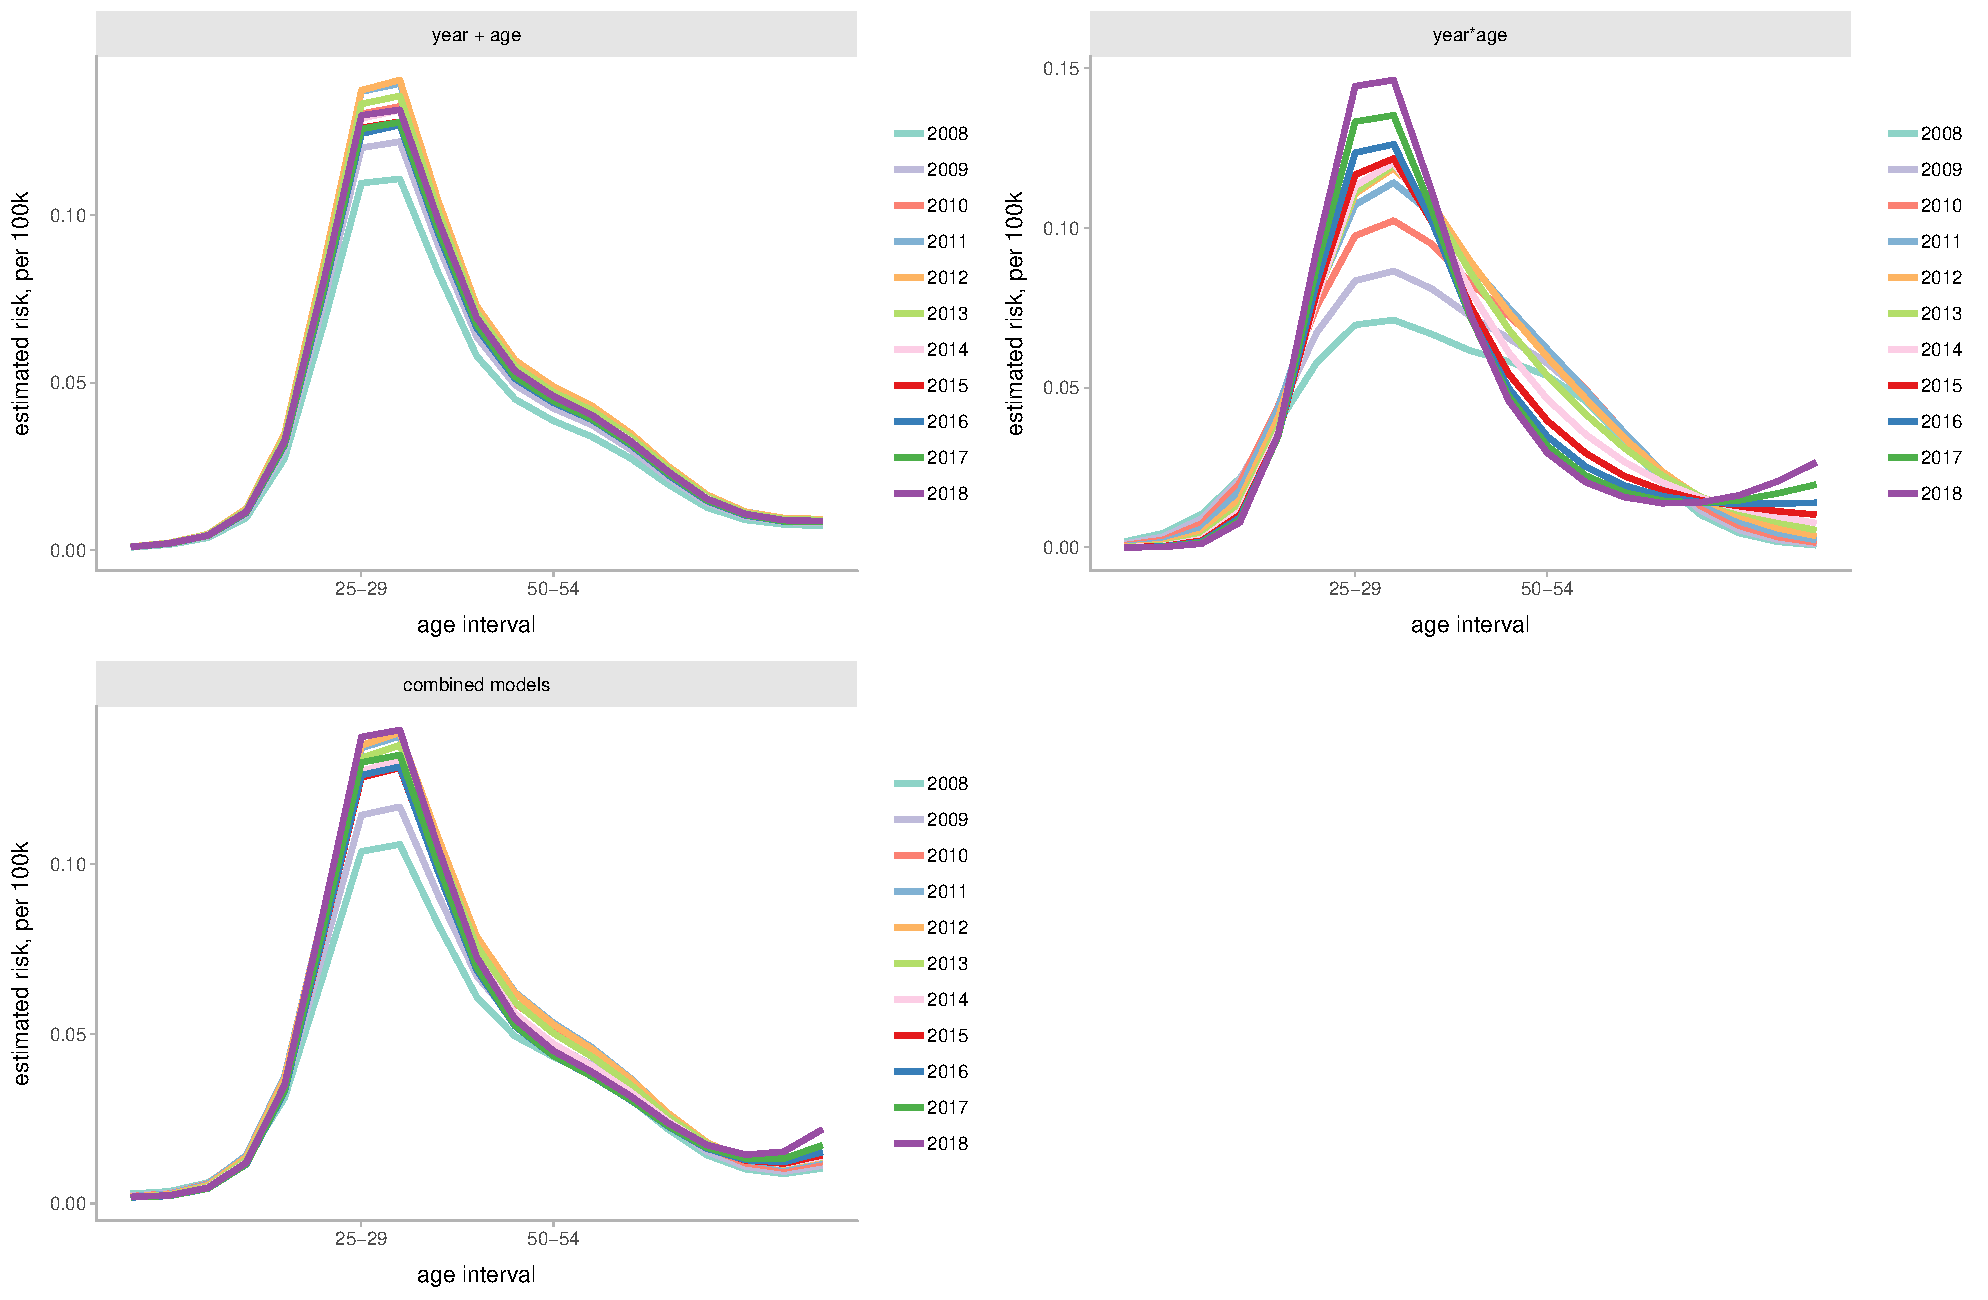
\includegraphics[width = \linewidth]{vis/fig_a4.pdf}
	\caption{Model estimated risk of police-mortality by age year for Black Females.}
	\label{fig:a4}
\end{figure}

The first panel of Figure \ref{fig:a4} gives predictions from Model A. Here, as expected, year shifts predicted mortality-risk upwards/downwards. The second panel, which gives predictions from Model B, shows that allowing year to modify age effects produces variation in estimates towards the tail-end of the life-course. (Predicted risk peaks around the same age-span for each year, but more risk exist among older ages during certain years in Model B.) The combined predictions, represented in the last panel, suggest that the year-by-age interaction is not strongly justified by the data. Indeed, the combined model almost entirely reduces to the predictions offered by Model 1. (Model 2 is given any weight as it appears to make a slight difference in predicting risk among the oldest age groups. The up-tick in risk during 2018 implied by Model B remains, to a degree, after combining models, for instance.) The intercept shift in risk across years appears to adequately describe the data. (Similar conclusions are drawn for every other group examined.)  

\subsection{Simulation models} 

With a better understanding of how time factors into our mortality estimates, we move to build the models that underline our life-table estimates. We fit and compare four specifications of how race, sex, age and year might predict risk of police-involved mortality. These specification are as follows: 

	\begin{align*}
		M_1\text{:} & \text{ death count} = f(\text{\text{race} + \text{sex} + age} + \text{year}) \\
		M_2\text{:} & \text{ death count} = f([\text{race}*\text{sex}] + \text{age} + \text{year}) \\
    M_3\text{:} & \text{ death count} = f([\text{race}*\text{sex}*\text{age}] + \text{year})   \\
		M_4\text{:} & \text{ death count} = f(\text{age} + [\text{race}*\text{sex}*\text{year}])   
	\end{align*}

Model 1 ($M_1$) assumes that race, sex, age and time have independent effects on mortality risk. Model 2 ($M_2$) allows for race and sex to jointly predict mortality, while Model 3 ($M_3$) allows for race and sex effects to further vary by age. Model 4 ($M_4$) allows for race and gender effects to vary by year. All models are multilevel, with race and sex fixed-effects and age-group and year specific-intercepts specified throughout. Log population size is used as an offset in each model. 

To determine which model best describes the data, we use leave-one-out-cross-validation information criterion (LOO-IC) estimates (Vehtari et. al. 2017). LOO-IC estimates are calculated from approximate leave one out cross-validation tests and broadly summarize a model's accuracy in predicting new data---relative to other model specifications. Like other information criterion measures (e.g., AIC; BIC), lower LOO-IC values indicate better fitting models. Table 1 gives LOOIC for each of the models described above: 

\begin{table}[H]
\centering
  \begin{tabular}{ccc}
    model & $\text{LOO-IC}$ \\ 
  \hline
    M0 & 4862.8 \\ 
    M1 & 4828.4 \\
    M2 & 4647.8 \\
    M3 & 4812.2 \\
  \hline
  \end{tabular}
  \caption{Model LOO-ICs}
\end{table}

Among the model specifications tested, M2 appears to fit the data the best. Indeed, when combining models via stacking weights, M2's posterior is assigned 100 percent of the prediction weight. We simulate from this model as such. 

\section{Race/ethnicity data in Fatal Encounters}

Fatal Encounters codes decedent race with the mutually exclusive values: African American/Black; Asian/Pacific Islander; European-American / White; Hispanic / Latino; Middle Easter; Native American / Alaskan; and Race unspecified. Ethnicity is not coded separately from race, so no distinctions among ethnic groups (i.e. Black and non-Black Latinx people) are possible using these data. We preserve these categories in all analyses, with the exception of Middle Eastern, which we recode to "White" based on census racial classifications to match population data. 

Fatal Encounters codes race/ethnicity opportunistically based on a series of potential data sources. When available, official records or news reports that explicitly identify a victim's race or ethnicity are used. However, such identifications are rare in news reports, which typically adhere to style guidelines limiting the use of racial or ethnic categories in their reporting. When explicit identifications are unavailable, Fatal Encounters researchers combine information and photos from original news reports, obituaries, or social media profiles to make qualitative assessments of a victim's race and ethnicity. 

Like overall counts of cases in Fatal Encounters, earlier years recorded in the data are likely subject to diminished quality due to the gradual development of internet news coverage, the timing of the development of major social media platforms, and the development of online obituary services, that made photos of individuals not directly included in news stories more widely available. We show a time series of the proportion of cases missing race/ethnicity data in FE in Figure \ref{fig:missing_race_ts}.

\begin{figure}
	\centering
	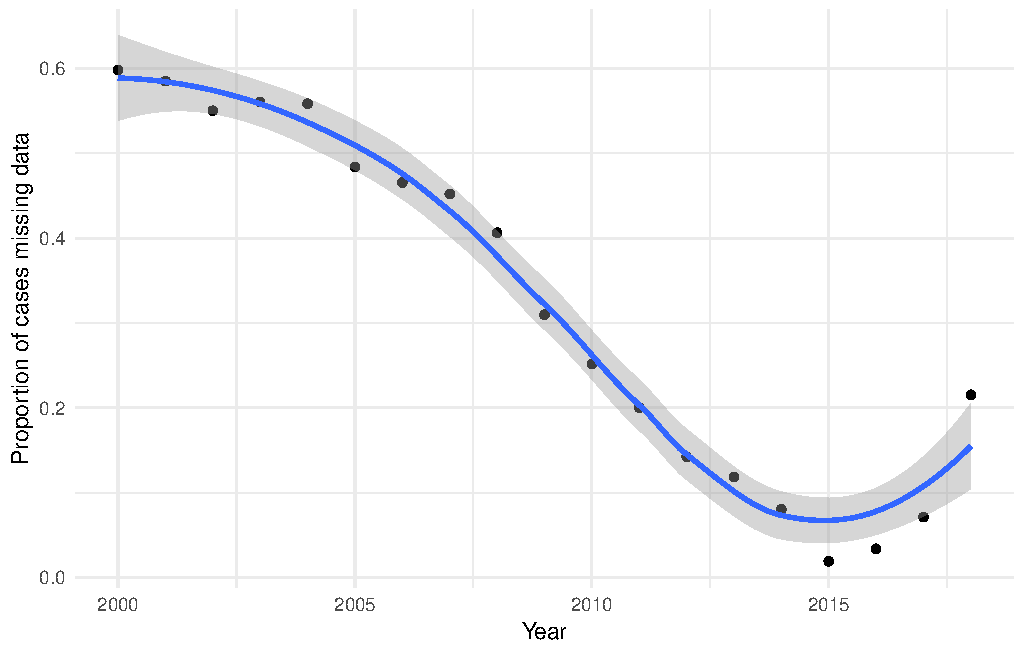
\includegraphics[width=\linewidth]{vis/prop_missing_race.pdf}
	\caption{Proportion of cases missing data on race/ethnicity in Fatal Encoutners, 2000 - 2018}
	\label{fig:missing_race_ts}
\end{figure}

About 60 percent of cases documented for 2000 are missing data on race/ethnicity. This proportion decreases steadily toward a minimum of about two percent of cases in 2015, followed by a gradual increase in recent years. Fatal Encounters researchers return to cases previously coded only based on news reports to conduct additional searches for obituaries published after the initial incident. In conversation with the authors, Fatal Encounters indicated that missing race/ethnicity data for 2018 and 2019 should be reduced once researchers conduct obituary searches for cases ocurring in these years.

\subsection{Comparing Fatal Encounters to NVSS data on race/ethnicity}

To evaluate the validity of Fatal Encounters race/ethnicity data, we again turn to the NVSS. If we assume that each racial / ethnic group has a similar probability of being recorded as a ``legal intervention'' death, conditional on being killed by police, then the relative case composition of legal intervention deaths in NVSS can be used to detect systematic bias in Fatal Encounters' race/ethnicity data. Below, we present the composition of Fatal Encounters cases prior to any missing data imputation procedures to ensure direct comparisons between the data recorded in each source.

\begin{figure}
	\centering
	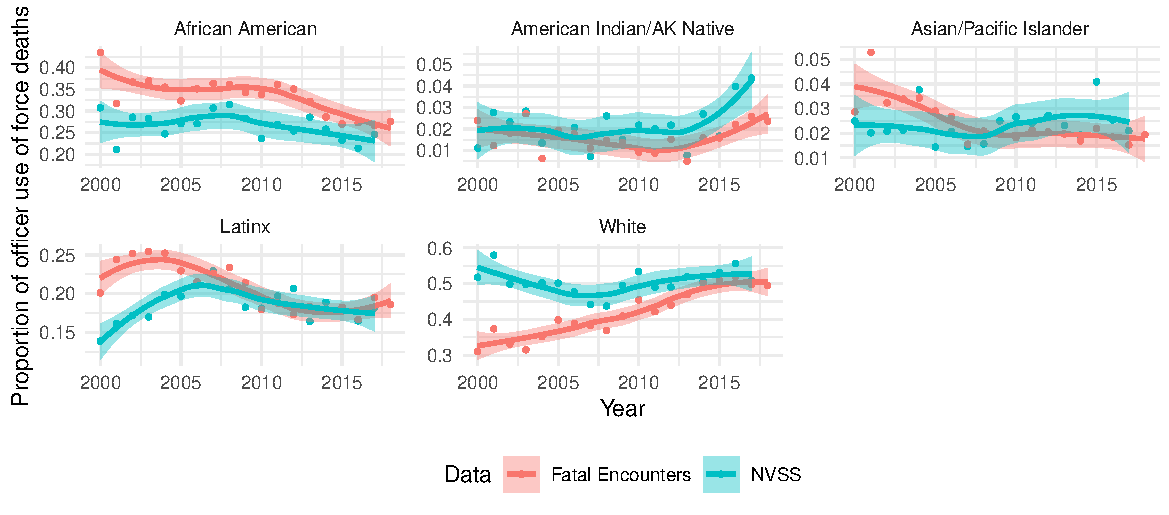
\includegraphics[width = \linewidth]{vis/fe_nvss_race_compare_na_rm.pdf}
	\caption{Proportion of cases in NVSS and Fatal Encounters by race, excluding cases missing race/ethnicity data, 2000 - 2018. Note that y-axis scales vary for each plot}
	\label{fig:compare_missing_na_rm}
\end{figure}

Figure \ref{fig:compare_missing_na_rm} shows the case composition by race/ethnicity excluding cases missing race/ethnicity data from the total case count in the proportion denominator. Note that there are no ``legal intervention'' cases missing race/ethnicity data in the NVSS. Both Fatal Encounters and NVSS record similar proportions of Asian / Pacific Islander victims. Until 2010, FE and NVSS record similar shares of American Indian victims, but NVSS records a greater share of American Indian / Alaska Native cases than does FE after 2010. Latinx victims made up a greater share of Fatal Encounters cases prior to 2008, but Latinx compositions appear similar across the datasets between 2008 and 2017. African Americans make up a consistently larger share of the case composition in Fatal Encounters than in NVSS. Among non-missing cases, Black victims composed between 40 and 28 percent of the caseload between 2000 and 2018. White victims ranged between 30 and 50 percent of the cases in Fatal Encounters, while NVSS consistently reports a white case composition of between 45 and 60 percent. The difference in case compositions between FE and NVSS for both white and Black victims diminishes between 2010 and 2017.

If the probability of being recorded as a ``legal intervention'' death in NVSS, conditional on being killed by police, is independent of race/ethnicity, then these analyses suggest that there may be some bias in documentation of race/ethnicity in Fatal Encounters. However, lacking external data known to be valid, this is an untestable assumption. It is possible that the evidence used by FE researchers to code race/ethnicity -- photographs, social media profiles, names, and obituaries -- affect the distribution of coded race/ethnicity data. 

Fatal Encounters researchers note that they have most confidence in their race/ethnicity data for data years after 2013. Between 2013 and 2017 (the latest available NVSS data), Fatal Encounters African American case composition was between 8 and 28 percent higher than NVSS, the American Indian / Alaska Native case composition was between 6 and 44 percent lower than NVSS, the Asian Pacific Islander caseload was between 12 and 46 percent lower than NVSS, the Latinx caseload was between 5 percent lower and 12 percent higher than NVSS, and the white caseload was between 1 and 9 percent lower than NVSS. 

It is important to note that FE records as many or more deaths than NVSS for each racial / ethnic group during this time period. Between 2013 and 2017, FE records $2549$ more cases than does NVSS (excluding the $364$ cases missing race ethnicity data during this period). Between 2008 and 2012, FE records more cases than does NVSS for all groups other than American Indian / Alaska Natives. In 2008, 2010, and 2011, FE records 3 fewer American Indian / Alaska Native deaths than does NVSS. In 2009 and 2012, FE records 2 more deaths than does NVSS. 

This comparison shows that FE racial/ethnic case compositions have some divergence from NVSS case compositions, and that these differences ar most pronounced for African Americans, American Indians, and Asian / Pacific Islanders. Despite these divergences, FE is generally recording dramatically more cases for each subgroup than is NVSS. Future researchers may consider conducting a systematic audit of FE race/ethnicity coding to evaluate the interrater reliability of FE coding decisions.

Of course, these analyses exclude missing cases. We further explore relationships between FE and NVSS race/ethnicity data in the context of missing data imputation in section 5. 

\section{Multiple imputation of missing data in Fatal Encounters}

Table \ref{tab:pct_var} shows the percent of cases missing data on each variable in Fatal Encounters between 2008 and 2018 for all causes of death, including suicides and non-use-of-force related deaths. Because we have reason to believe that case counts are censored in earlier years of the data, we exclude observations from 2000 to 2007 in imputation models. About 3 percent of cases are missing data on victim age, about 0.3 percent are missing data on victim sex, about 21 percent are missing data on victim race, and less than one percent are missing data on the cause of death. 

% latex table generated in R 3.5.2 by xtable 1.8-3 package
% Wed Mar  6 19:46:07 2019
\begin{table}[ht]
\centering
\begin{tabular}{rrrr}
  \hline
Age & Sex & Race & Cause of death \\ 
  \hline
3.050 & 0.349 & 21.200 & 0.006 \\ 
   \hline
\end{tabular}
\caption{Focal variables missing values in Fatal Encounters, percent of cases 2008 - 2018} 
\label{tab:pct_var}
\end{table}


To address missing data, we draw multiple imputations of missing values based on models including information on the year of death, victim age, victim sex, victim race, the cause of death, the racial composition of the county in which the victim was killed, and the probability of a victim's race/ethnicity conditional on victim surname compiled from Census surname lists by Imai and Khana (CITE). Sensitivity analyses exploring the predictive validity of county, tract and block-group-level demographics suggested that county-level demographics maximized model classification validity. This is perhaps due to the fact that geodata recorded in Fatal Encounters records the location of death, and many victims recorded in Fatal Encounters did not die at home. Home addresses would provide greater utility in predicting victim race/ethnicity, but are not available. 

Multiple imputation enables us to model uncertainty in the composition of cases in Fatal Encounters driven by missing data through the construction of uncertainty intervals derived from samples from our missing data models. These count estimates are by definition equal to or greater than those directly estimated from the observed data. However, by making the assumption that values are missing at random conditional on model predictors, we are able to provide additional precision in estimating the range within which actual mortality risk lies for each subgroup. 

Model predictions are generated using multiple imputation through chained equations (CITE VAN BUUREN). We construct 50 imputed datasets to ensure adequate coverage of uncertainty intervals for the race variable, which has a high number of missing cases in earlier years of the data. 

Figure \ref{fig:traceplot} shows the estimated mean and standard deviation of each imputed dataset (color) by variable across iterations, using an Markov Chain Monte Carlo based approach to imputing predicted values in resulting datasets. The traceplots indicate model convergence, and appear free of any trends. 

\begin{figure}
	\centering
	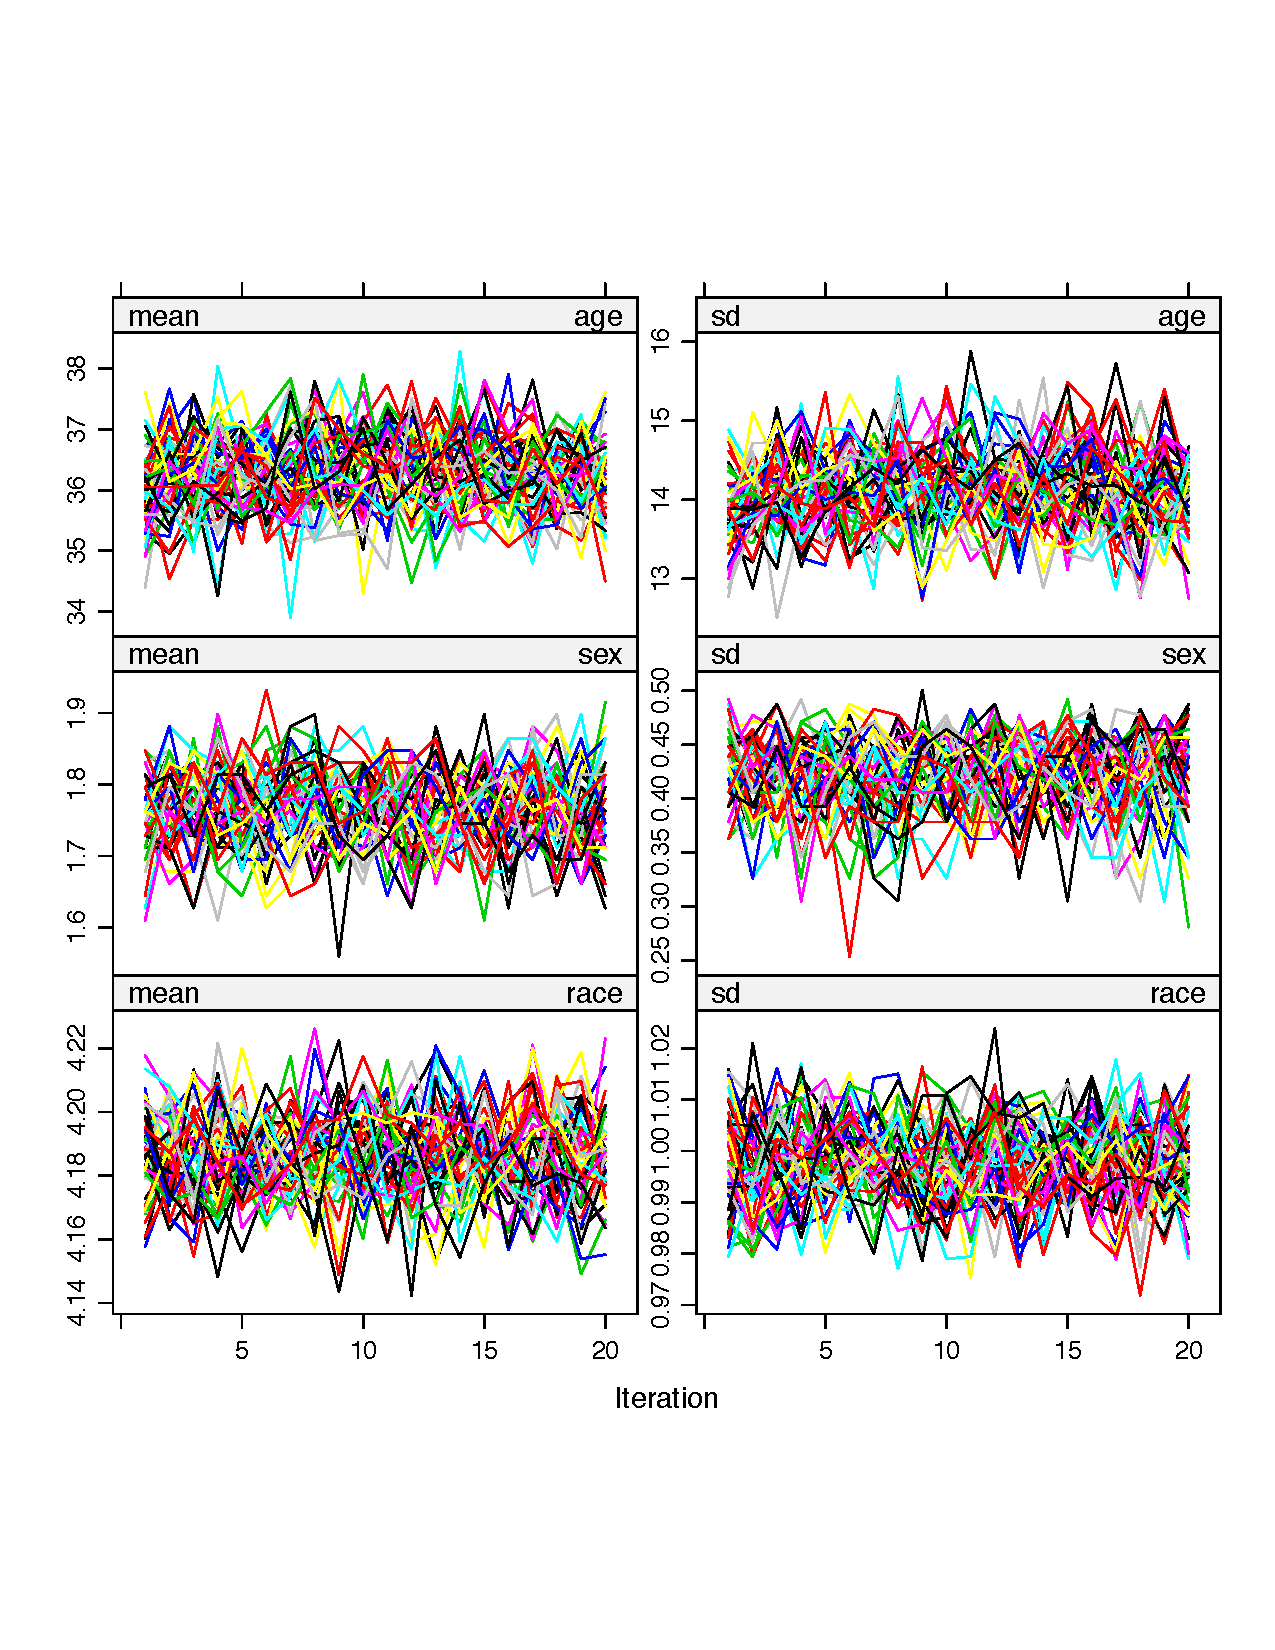
\includegraphics[width = \linewidth]{vis/imp_trace_1.pdf}
	\caption{Traceplot of mean and standard deviation of imputed variables}
	\label{fig:traceplot}
\end{figure}

\begin{figure}
	\centering
	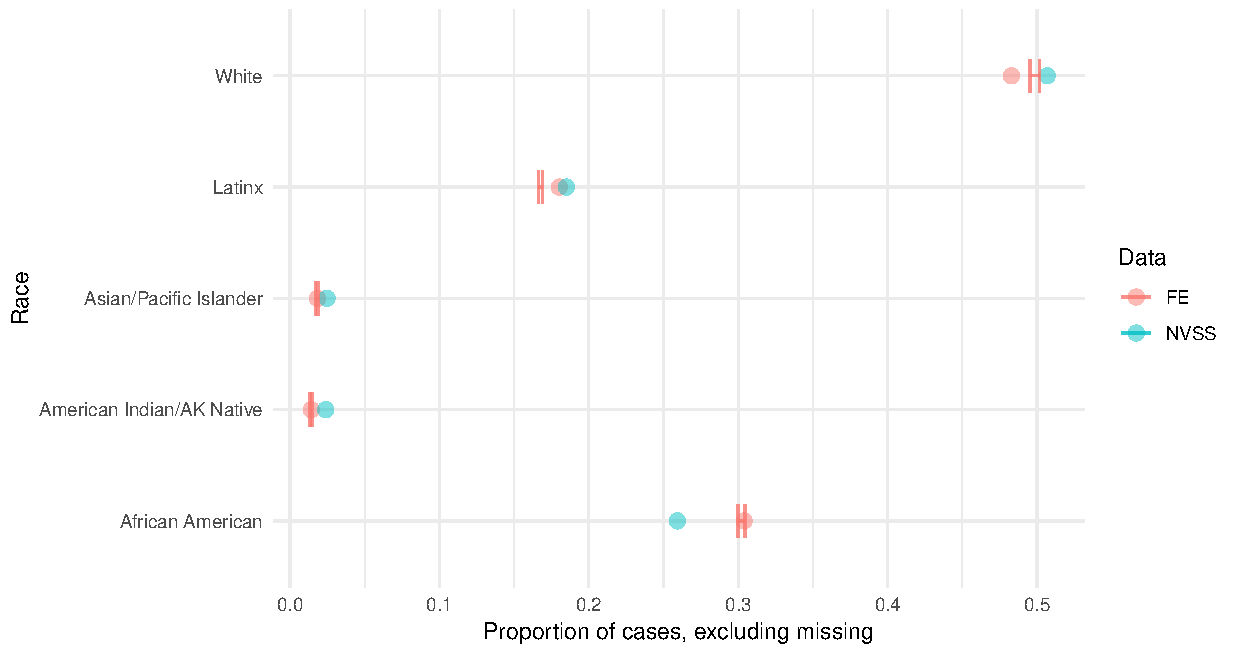
\includegraphics[width = \linewidth]{vis/race_impute_pct.pdf}
	\caption{Proportion of cases in observed Fatal Encounters and NVSS data (point) and range of imputed data (bar), 2008 - 2018}
	\label{fig:race_impute_pct}
\end{figure}

We show the distribution of the imputed race/ethnicity variable relative to the observed data in Figure \ref{fig:race_impute_pct}. The solid points in this figure represent the observed proportion of cases in each group, and the bars represent the range of the imputed values. For American Indian, Asian, and Black people, the proportion of the observed FE data in each group is within the range of the imputed values. The distribution of the imputed data do not greatly differ than the distribution of the observed data for these groups. There is a greater share of Latinx victims in the observed data than there are in the imputed data, and there is a greater share of white victims in the imputed data than there are in the observed data. 

In the observed data (excluding missing cases), Latinx victims make up about 18 percent of the recorded cases. Our imputations suggest that they make up between 16.7 and 16.9 percent of all cases. White victims make up about 48 percent of the recorded cases in the observed data. Our imputations suggest they make up between 49.5 and 50.1 percent of all cases. 

This gap between imputed and observed proportions in Fatal Encounters is a function of the relationship between the probability of missingness and a victim's race/ethnicity. Our imputation models address this dependence by including two direct predictors of victim race/ethnicity; victim surname and racial/ethnic population composition in the county of death. 

% latex table generated in R 3.5.2 by xtable 1.8-3 package
% Wed Feb 27 15:47:58 2019
\begin{table}[H]
\centering
\begin{tabular}{lrr}
  \hline
Term & Estimate & SE \\ 
  \hline
County proportion American Indian & 0.20 & 0.45 \\ 
  County proportion Asian & -0.24 & 0.34 \\ 
  County proportion Black & -0.04 & 0.16 \\ 
  County proportion Hispanic & -0.96 & 0.16 \\ 
  Pr(White$|$Surname) & -1.06 & 0.54 \\ 
  Pr(Black$|$Surname) & -0.97 & 0.57 \\ 
  Pr(Hispanic$|$Surname) & -1.16 & 0.54 \\ 
  Pr(Asian$|$Surname) & -0.85 & 0.59 \\ 
   \hline
\end{tabular}
\caption{Relationships between county racial demographics,
         surnames and likelihood of missing race/ethnicity data in Fatal Encounters 2000 - 2018.
         Logistic regression with year intercepts, age slope, sex intercept, and
         cause of death intercept estimated but not displayed.} 
\label{tab:missing_reg}
\end{table}


To evaluate whether these predictors are correlated with missingness, we model the probability that a case is missing race/ethnicity data with a logistic regression. Selected parameter estimates from this model are displayed in Table \ref{tab:missing_reg}. Cases are less likely to be missing data when they are in counties with large Hispanic populations than when they occur in counties with smaller Hispanic populations. A surname with a high conditional probability of being Hispanic based on census records is also associated with a a lower probability of being missing. These relationships suggest that names and locations of death are associated with a higher likelihood of positive ethnic identification in Fatal Encounters, either through identifying features in initial reports, or through coder inference based on surname or other contextual information. Because Latinx victims are less likely to be missing in the observed data, their share of total reports in imputed data is somewhat lower. 

\subsection{Sensitivity of risk estimates to missing data and period choice}

Our estimates of the lifetime risk of being killed by police are sensitive to the imputation of missing race/ethnicity data and to the choice of period included in lifetable estimates. Below, we present results from lifetables calculcate using only the observed and imputed data. These estimates are not based on the model-based simulations presented in the manuscript. ADD IN AN X FOR THE MODEL PREDS IN THIS FIG!!!!!!

\begin{figure}[H]
	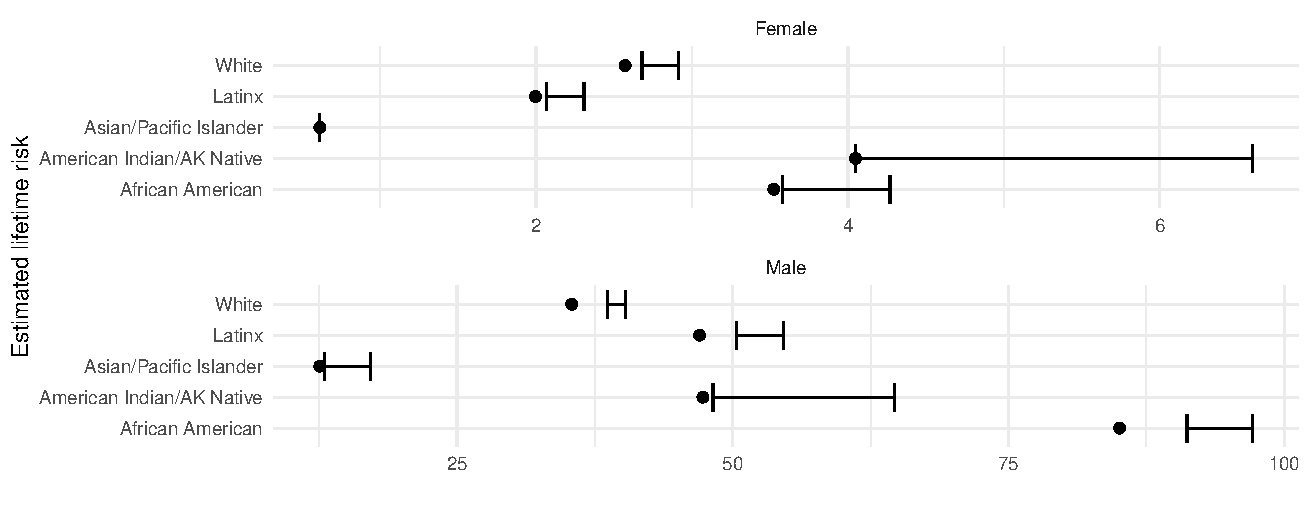
\includegraphics[width=\linewidth]{vis/imp_period_sensitivity.pdf}
	\caption{Sensitivity of risk estimates to missing data and period choice}
\end{figure}


\section{Inclusion criteria and mortality estimates}

\begin{figure}
	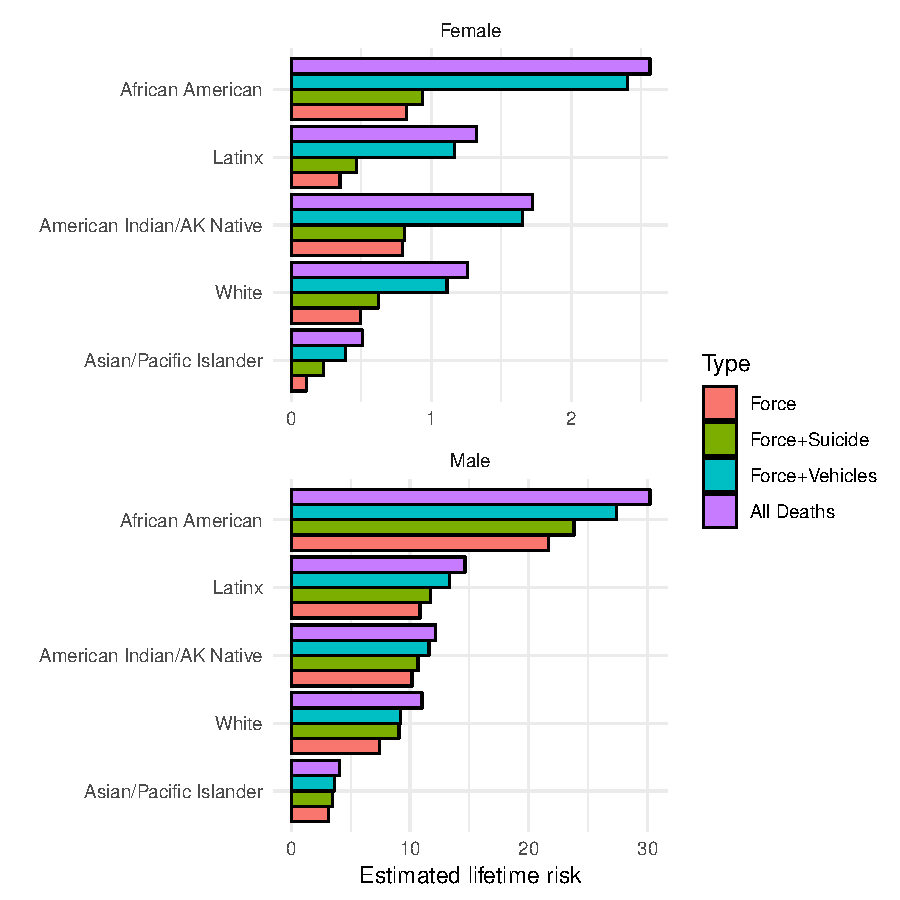
\includegraphics[width=\linewidth]{vis/death_type_c.pdf}
	\caption{Cumulative risk of dying during interactions with law enforcement by race, sex, and cause of death}
	\label{fig:death_type}
\end{figure}

\section{Complete life tables}

demo the lifetable with one group

then show abridged life tables for each group

\end{document}
